\documentclass{article}
\usepackage{biblatex} %Imports biblatex package
\addbibresource{refs.bib} %Import the bibliography file
\usepackage{minted, float, booktabs}
\usepackage{subfig}
\usepackage{url}
\usepackage[utf8]{inputenc}
\setlength\parindent{0pt}
\usepackage{parskip} 
\usepackage{geometry}
 \geometry{
 a4paper,
 total={170mm,257mm},
 left=30mm,
 right=30mm,
 top=30mm,
 bottom=30mm,
 }
 \usepackage{graphicx}
 \usepackage{titling}
 \usepackage{amsmath,amsfonts,amssymb,amsthm,float}

\title{Clonal Lineage Analysis of Antibody Repertoire Seq Data}
\author{Dohyoung Ko}
\date{November 15 2024}
 
 \usepackage{fancyhdr}
\fancypagestyle{plain}{%  the preset of fancyhdr 
    \fancyhf{} % clear all header and footer fields
    \fancyfoot[L]{\thedate}
    \fancyfoot[R]{Page \thepage \hspace{1pt}}
    \fancyhead[L]{Assignment 3}
    \fancyhead[R]{\theauthor}
}
\makeatletter
\def\@maketitle{%
  \newpage
  \begin{center}%
  \let \footnote \thanks
    {\huge \@title \par}%
    \vskip 2em%
    {\large Dohyoung Ko}%
    \vskip 1em%
    {Department of Computer Science and Engineering, The Pennsylvania State University}
    \vskip 1em%
    {\@date}
  \end{center}%
  \par
  \vskip 1em}
\makeatother

\usepackage{cmbright}

\newcommand{\abs}[1]{\left\lvert #1 \right\rvert} % absolute value 

\begin{document}

\renewcommand{\theFancyVerbLine}{
  \sffamily\textcolor[rgb]{0.5,0.5,0.5}{\scriptsize\arabic{FancyVerbLine}}}


\maketitle

\section*{\centering Abstract}
This report offers a comprehensive examination of the clonal lineage analysis of antibody repertoire sequencing data obtained post-seasonal influenza vaccination. It discusses the rationale and computational framework under each phase of antibody repertoire sequencing data analysis and analyzes the findings of the experiment. Germline V, D, and J gene alignments to the antibody repertoire sequencing data were identified, and the CDR3 antigen-binding region for each query sequence was delineated using the National Center for Biotechnology Information (NCBI)'s IgBLAST software. Subsequently, the clonal lineage was deduced by evaluating the connected components of the Hamming graph constructed from this IgBLAST analysis. All computational processes for the analysis were executed on the Cedar heterogeneous cluster at Simon Fraser University as part of the Advanced Research Computing service provided by the Digital Research Alliance of Canada. The code utilized for the analysis is accessible on GitHub(\url{https://github.com/kodh49/antibody_repertoire.git}).

\hfill

\tableofcontents

\hfill


\section{Antibody Repertoire Sequencing Data}
Prior to reconstructing clonal lineages within an antibody repertoire, we performed an NCBI IgBlast analysis to preprocess the database. This step is to identify germline V, D, J gene matches and antigen binding regions, most importantly CDR3, from the given database. The NCBI IgBlast tool offers such functionality. It is available on the web, but this analysis used the standalone version for an integrated analysis environment. The antibody repertoire employed in this analysis is accessible through the following link (\url{https://drive.google.com/file/d/1RUzTU62V4C0rV_EzSDMfZlaMWc_7Cc3z}). This database comprises 10,000 sequences obtained subsequent to a seasonal influenza vaccination.

\subsection{IMGT Database Construction}
The first step is to construct reference germline database that will be used for VDJ gene matching and CDR3 identifications. In this experiment, we searched IMGT germline sequences available fromIMGT web site (\url{http://www.imgt.org/vquest/refseqh.html#VQUEST}). Since the database is conducted on Homo Sapiens, we used all pre-annotated V, D and J sequences for human category. We combined all V, all D and all J sequences, respectively, into separate files (i.e., one file for all V sequences, one for all D sequences and one file all for J sequences). The following command invokes the utility tool \texttt{edit\_imgt\_file.pl} in the bin directory of the IgBlast release package to process these sequences (i.e., to change the long IMGT definition lines to germline gene names only). For instance,
\begin{minted}{shell}
    bin/edit_imgt_file.pl my_seq_V > my_seq_V
\end{minted}
By running the following command, \texttt{makeblastdb} tool provided by NCBI constructs the blast database from the above output file.
\begin{minted}{shell}
    bin/makeblastdb -parse_seqids -dbtype nucl -in my_seq_V
\end{minted}
We repeat the above process to all V, D, and J fasta files to construct three separate blast database files to be used by IgBlast later.

\subsection{NCBI IgBlast Analysis}
Using this reference database, we performed the IgBlast analysis through the Cedar heterogeneous cluster located at Simon Fraser University as part of the Advanced Research Computing service offered by the Digital Research Alliance of Canada. The following script is used to run the analysis using the default auxiliary data provided by NCBI.
\begin{minted}{shell}
    # Define input and output paths
    QUERY="data/PRJNA324093_Dnr4_10k.fasta"
    OUTPUT="data/igblast_results.tsv"
    DB_DIR="database"
    AUXILIARY="optional_file/human_gl.aux"
    CORES=48
    
    # run ncbi-igblash-1.22.0
    bin/igblastn -germline_db_V $DB_DIR/my_seq_V
                 -germline_db_D $DB_DIR/my_seq_D
                 -germline_db_J $DB_DIR/my_seq_J
                 -organism human
                 -domain_system imgt
                 -query ../$QUERY
                 -outfmt 19
                 -out ../$OUTPUT
                 -auxiliary_data $AUXILIARY
                 -num_threads $CORES
\end{minted}

\subsection{Hamming Graph}
For an in depth analysis of antibody repertoire and clonal lineages, we computed a Hamming graph on the computed CDR3s. In this graph, each unique CDR3 region represents a vertex, and two CDR3s are connected with an edge if it all satisfies the following three conditions.
\begin{enumerate}
    \item Two CDR3s have the equal length.
    \item the Hamming distance between their nucleotide sequences is below 10\%.
    \item Two CDR3s represent VDJ sequences with identical V and J genes.
\end{enumerate}
We ignored gene alleles while checking the third condition. For example, we assumed that alleles IGHV1-69*01 and IGHV1-69*02 represent the same gene. The Hamming distance between two nucleotide sequences $A$ and $B$ of equal length $n$ is computed as the following.
\begin{align}
    d(A,B) = n -\sum_{i=1}^n \delta(A_i,B_i)
\end{align}
where $\delta$ is a Kronecker delta function.

\section{Clonal Lineage Analysis}
This section will discuss the implementation and interpretation of clonal lineage analysis based on the Hamming graph formulation of the VDJ aligned immunoglobins data. In this formulation, connected components of the computed Hamming graph represent clonal lineages of the data. Table \ref{table:clonal_summary} summarizes some of the important statistics obtained from the clonal lineage analysis.
\begin{table}[H]
\centering
\begin{tabular}{lc}
\toprule
Category & Statistics \\
\midrule
Number of Clonal Lineages & 623 \\
Number of Sequences in the Largest Lineage & 501 \\
Number of Clonal Lineages presented by at least 10 Sequences & 272 \\
\bottomrule
\end{tabular}
\caption{Clonal Lineages Summary}
\label{table:clonal_summary}
\end{table}
Figure \ref{fig:clonal_stats} provides a more extensive statistics regarding the clonal lineage analysis such as the number of unique CDR3 regions in the largest clonal lineage and the number of lineages represented by at least 10 unique CDR3 regions. Since we accounted for the error in sequencing by identifying a connection between two CDR3 regions whenever their hamming distance is less than 10\% of its length, there are more full sequences, i.e. 501 sequences, attached to a particular clonal lineage than CDR3s, which are only 103 CDR3 regions.
\begin{figure}[H]
    \centering
    
\includegraphics[width=0.7\linewidth]{clonal_lineage_stats.png}
    \caption{Clonal Lineages Statistics}
    \label{fig:clonal_stats}
\end{figure}


\subsection{V Gene Usage}
This subsection elaborates on the usage of V genes in the original data to the antibody repertoire. Figure \ref{fig:v_gene_usage} showcases the usgae plot of the computed V genes in the sample data. The $x$-axis represent each V gene in the sample, and $y$-axis represent the number of clonal lineages formed by each of V genes.
\begin{figure}[H]
    \centering
    
\includegraphics[width=0.8\linewidth]{usage_plot.png}
    \caption{Plot of V Gene Usage}
    \label{fig:v_gene_usage}
\end{figure}
The following table provides a more comprehensive view of the six main V genes that appeared the most in across all clonal lineages.
\begin{table}[H]
\centering
\begin{tabular}{lc}
\toprule
IMGT Label & Lineage Count \\
\midrule
IGHV3-23 & 979 \\
IGHV3-23D & 964 \\
IGHV3-7 & 769 \\
IGHV3-30 & 768 \\
IGHV3-15 & 732 \\
IGHV1-2 & 719 \\
\bottomrule
\end{tabular}
\caption{Top six V genes in clonal lineages}
\label{table:normalization_count}
\end{table}
The above analysis does not account for alleles of these genes. Note that these genes that are highly involved in clonal lineages correspond to the V region of the variable domain of immunoglobulin heavy chains that participates in antigen recognition. Most of the main genes are from the IGHV3 family. For example, IGHV3-23 belongs to a cluster of approximately 40 functional variable (V) genes in the immunoglobulin heavy chain locus on chromosome 14.

\subsection{Amino Acid Sequences}
Figure \ref{fig:weblogo_plot} presents the weblogo plot of amino acid sequences of CDR3s from the largest clonal lineage.
\begin{figure}[H]
    \centering
    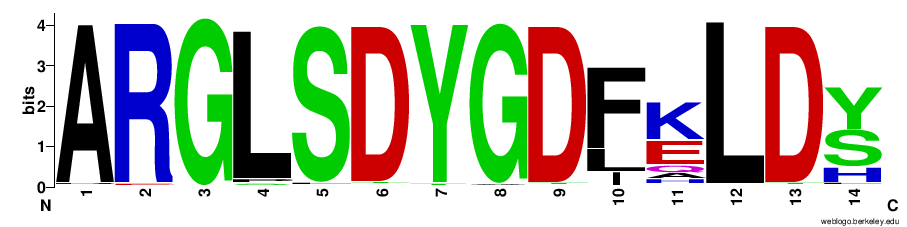
\includegraphics[width=0.8\linewidth]{weblogo.png}
    \caption{Weblogo Plot}
    \label{fig:weblogo_plot}
\end{figure}
\end{document}